% ============================================================================
% 中文注释：第 1 节 引言（2026-11-03 第三版）——按标准论文结构重写
% ----------------------------------------------------------------------------
% 结构（用户指定）：
%   ① 背景：SIRR 是什么、用在哪些场景、主流方法解决了什么
%   ② 痛点：真实部署里玻璃基本都贴膜；贴膜改变的成像；现有方法因此失效
%   ③ 前人方法：做过什么、进展到哪、仍缺什么
%   ④ 自己方法 + teaser（图 1 = 同权重 Real20 成功 / 贴膜失败）
%   ⑤ 核心贡献 5 条 bullet（数据 / 成像 / 区域分析 / 方法 / 负结果）
%   ⑥ 论文结构
% 写作纪律（用户要求）：
%   **intro 不写具体数字**，数字一律留给图表。
%   数据贡献必须写全：15 场景测试集 + 4/5/6/11 月四个训练批次。
% ============================================================================
\section{Introduction}
\label{sec:intro}

% 中文：图 1 —— 同一官方权重（RDNet CVPR'25），Real20 能去干净、贴膜场景去不掉。
\begin{figure*}[t]
\centering
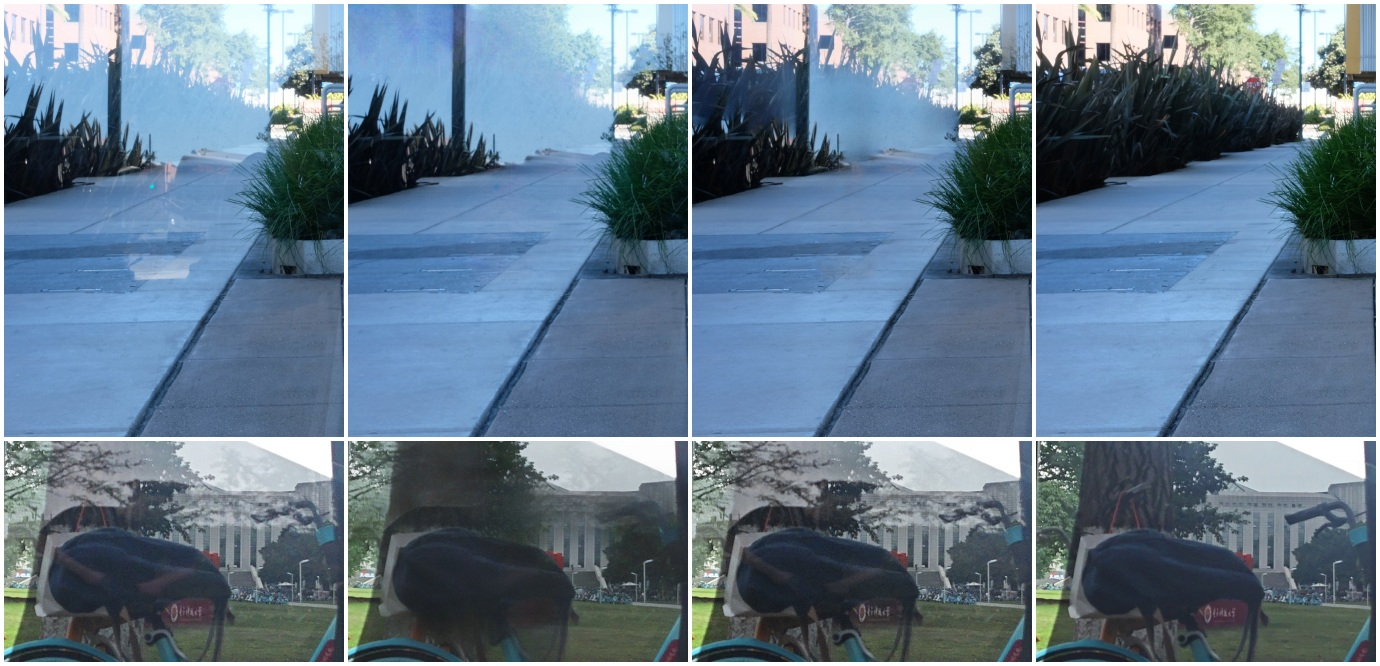
\includegraphics[width=0.86\textwidth]{fig/teaser_2rows.jpg}
\caption{\textbf{Same models, two kinds of glass.} Top, on a standard benchmark (Real20): the
state-of-the-art method~\cite{rdnet25} removes the reflection almost completely, while a second
recent method (LightRR~\cite{lightrr26}) removes only part of it. Bottom, on a pair from our
filmed-glass panel: the \emph{same} RDNet does not remove the reflection at all---instead it darkens
the frame and strips transmitted detail---and LightRR changes almost nothing. The difference is not
the network but the imaging: window film is laminated on the scene side, so the transmitted light
passes through the film while the reflection of the behind-camera environment does not. The two
layers end up separated in \emph{band} rather than in \emph{level}, and a model trained on ordinary
glass misreads what to take away.}
\label{fig:teaser}
\end{figure*}

% 中文：① 背景。
Single-image reflection removal (SIRR) addresses a situation everyone with a camera has met: a
photograph taken through a pane of glass, in which the scene behind the camera is superimposed on
the scene in front of it. The setting is ubiquitous---car windows, shop and office facades, museum
cases, aquaria---and the degradation is severe enough that SIRR has become a standing task in
computational photography. The dominant recipes are now data-driven: large paired corpora of
``with reflection / without reflection'' images, a network that regresses the transmitted layer, and
an objective that penalises the difference from the clean reference. Classical layer priors gave way
to cascaded and recurrent designs, then to reversible and dual-stream architectures, and each
generation has advanced the state of the art on benchmarks such as Real20 and SIR$^2$.

% 中文：② 痛点。真实部署 = 贴膜玻璃。
What these recipes share is an implicit assumption about the \emph{glass}. In deployment the glass
is rarely bare: automotive and architectural glazing is almost always \emph{filmed}, for heat
rejection, privacy and UV protection. A dark film changes the imaging in a way that the standard
assumption does not cover. The film sits on the scene side, so the light we want must travel through
it---and is scattered, absorbed and tinted on the way---while the light we want to discard comes off
the bare surface facing the camera and passes through nothing. The observed image is therefore not a
bright reflection layered on a well-exposed scene, but a \emph{sharp} reflection over a \emph{soft},
desaturated transmission. Methods trained on ordinary glass, and evaluated on ordinary glass, have no
reason to expect this, and empirically they do not survive it (Fig.~\ref{fig:teaser}).

% 中文：③ 前人方法：做过什么、缺什么。
The community has of course attacked the difficulty of SIRR from several directions: stronger
backbones and attention, reversible or invertible connections to preserve information, explicit
estimates of the reflection rate, physics-inspired layer decompositions, and larger or more realistic
synthetic corpora. What these efforts have in common is where they are measured: on benchmarks whose
reflections are \emph{dense}, covering most of the frame, so that an average error over the image is
already a faithful description of the failure. Three things are consequently missing. There is no
real paired dataset shot through filmed glass, so the regime cannot even be measured. There is no
analysis of \emph{where} a method fails---strong reflection is not distributed uniformly over the
frame, and a single average number cannot distinguish the regions where removal is necessary from
those where it is harmful. And because no such analysis exists, the losses used in training are
inherited from dense-reflection settings, where they work.

% 中文：④ 自己方法：先量清楚，再给监督。
This paper takes the opposite order. We first ask what filmed glass actually does to the two layers,
and answer it with measurements: the transmission loses high-frequency content relative to ordinary
glass while the reflection does not, so the layer that carries the detail and the layer that must be
discarded are separated in frequency rather than in brightness. We then ask \emph{where} current
methods fail, and find that the answer is unintuitive: the reflection is weakest exactly in the
region the eye fixates on---the patch where a dark object of the reflected environment projects,
which we call the low-change region---and strongest in the annulus immediately around it. The
annulus is large, its transmitted content is buried, and every model we tested is worse there than
anywhere else in the frame; because it borders a region that is already almost correct, its residual
error is read by the eye as a boundary. Finally, guided by this picture, we design the training
signal: a compact region with a large weight is what keeps a sparse reflection from being
under-weighted by the global objective, and this can be obtained without any annotation at all.
Along the way we capture the data that makes the analysis possible.

% 中文：⑤ 核心贡献。
\paragraph{Contributions.}
\begin{itemize}
\item \textbf{Data.} A real-pair benchmark for filmed glass: a hand-annotated test panel of
$15$ scenes, and training pairs captured in four sessions (April, May, June and November) on the
same rig with exposure and white balance locked. We also report the two capture pitfalls that
silently ruin such data---unlocked auto-exposure, which makes the ``clean'' reference a different
exposure of the scene, and misalignment between the pair---together with the protocol we use to
avoid them.
\item \textbf{Imaging.} A measurement-based account of filmed glass as a layer \emph{asymmetry}:
transmission through the film bulk, reflection off the bare surface. We show that the two layers
differ in band and in chroma, but not in mean level, which distinguishes filmed glass from ordinary
glass and explains why off-the-shelf models transfer poorly.
\item \textbf{Regional analysis.} A decomposition of the failure into the low-change region and the
annulus around it. The reflection is weakest inside the region and strongest in the annulus; models
are worse than doing nothing inside the region, and at their absolute worst in the annulus. This is
what makes the boundary, rather than either region on its own, the thing one sees.
\item \textbf{Method.} Evidence that region-relative supervision is load-bearing for sparse
reflection, and a mask-free change-aware regulariser, $\mathcal{L}_{\mathrm{quiet}}$, derived from
it: no annotation, no parameters, no inference cost, and a consistent improvement over our
fine-tuning baseline.
\item \textbf{Negative results.} A systematic account of what does \emph{not} work on this problem,
with a mechanism for each failure: perceptual losses, restoring the input's high frequencies,
mixing in more in-domain data, a photometric adapter, a residual gate, and a dual-dictionary
separation probe.
\end{itemize}

% 中文：⑥ 论文结构。
\paragraph{Organisation.}
Sec.~\ref{sec:related} reviews related work. Sec.~\ref{sec:benchmark} describes the imaging of
filmed glass, the capture protocol and the datasets. Sec.~\ref{sec:diagnosis} analyses where and why
current methods fail. Sec.~\ref{sec:method} derives the training signal, and
Sec.~\ref{sec:experiments} reports results, ablations and negative results.
Sec.~\ref{sec:conclusion} discusses limitations and the open problem of completing the annulus.
